\documentclass[titlepage,a4paper]{article}

\usepackage{a4wide}
\usepackage[colorlinks=true,linkcolor=black,urlcolor=blue,bookmarksopen=true]{hyperref}
\usepackage{bookmark}
\usepackage{fancyhdr}
\usepackage[spanish]{babel}
\usepackage[utf8]{inputenc}
\usepackage[T1]{fontenc}
\usepackage{graphicx}
\usepackage{float}

\pagestyle{fancy} % Encabezado y pie de página
\fancyhf{}
\fancyhead[L]{TP1 - Carlos Castillo}
\fancyhead[R]{Algoritmos y Programación III - FIUBA}
\renewcommand{\headrulewidth}{0.4pt}
\fancyfoot[C]{\thepage}
\renewcommand{\footrulewidth}{0.4pt}

\begin{document}
\begin{titlepage} % Carátula
	\hfill\includegraphics[width=6cm]{logofiuba.jpg}
    \centering
    \vfill
    \Huge \textbf{Trabajo Práctico 1 — Smalltalk}
    \vskip2cm
    \Large [7507/9502] Algoritmos y Programación III\\
    Curso 2
    Primer cuatrimestre de 2022 
    \vfill
    \begin{tabular}{ | l | l | } % Datos del alumno
      \hline
      Alumno: & CASTILLO, Carlos Eduardo \\ \hline
      Número de padrón: & 108535 \\ \hline
      Email: & ccastillo@fi.uba.ar \\ \hline
  	\end{tabular}
    \vfill
    \vfill
\end{titlepage}

\tableofcontents % Índice general
\newpage



\section{Introducción}\label{sec:intro}
El presente informe reune la documentación de la solución del primer trabajo práctico de la materia Algoritmos y Programación III que consiste en desarrollar una aplicación de un sistema telefónica de registro y cobro de llamadas en Pharo utilizando los conceptos del paradigma de la orientación a objetos vistos hasta ahora en el curso.



\section{Supuestos}\label{sec:supuestos}
% Deberá contener explicaciones de cada uno de los supuestos que el alumno haya tenido que adoptar a partir de situaciones que no estén contempladas en la especificación.

Si bien la especificación otorgada brinda información general del comportamiento esperado del sistema desarrollado, hay cierto aspecto del funcionamiento del mismo que no han sido aclarados en dicha especificación. Debido a esto se han hecho las siguientes suposiciones:

\begin{itemize}
  \item El abono mensual de una línea telefónica se establece al momento de creación de dicha línea, por lo tanto no hay forma de cambiar este valor a menos que se cree una línea nueva.
  \item Una vez que se ha registrado una llamada no hay forma de modificar los datos de la llamada registrada. En efecto, tampoco hay forma de acceder a ninguna de las llamadas del registro individualmente, mucho menos de modificar dichas llamadas.
  \item El rango de horas considerado como horario laboral es el mismo para todas las línea y no puede ser modificado.
  \item La tarifa por minutos de las llamadas internacionales puede ser cero. Una situación en la que se podría utilizar este comportamiento es, por ejemplo, para promociones de llamadas internacionales gratuitas.
  \item El descuento a llamadas nacionales de larga duración también aplica para llamadas internacionales de larga duración.
  \item Al momento de determinar si una llamada fue realizada dentro del horario laboral, únicamente se toma en cuenta el horario de inicio de la llamada, sin importar su duración (con lo que se estaría tomando más bien el horario de finalización). Por ejemplo, si una llamada es hecha a las 19 horas (dentro del horario laboral), pero tiene una duración de 120 minutos, terminando a las 21 horas (fuera del horario laboral), igualmente es cobrada como llamada realizada dentro del horario hábil.
\end{itemize}



\section{Modelo de dominio}\label{sec:modelo}
% Explicación concisa del diseño general del trabajo.

La entidad principal del problema es una línea telefónica cuya funcionalidad es básicamente registrar y cobrar llamadas.
Toda un abono mensual, que es un mínimo constante que se abona mes a mes, independientemente de que se hayan registrado llamadas o no a lo largo de ese mes.

Las llamadas que se pueden registrar en una línea telefónica pueden ser llamadas nacionales o internacionales. Ambos tipos de llamadas tienen una duración y un horario en que fueron realizadas. Adicionalmente, las llamadas internacionales tiene un destino específico. Todas las llamadas tienen una tarifa por minuto, que en el caso de las llamadas nacionales, varía en base a si dicha llamada fue realizada dentro del rango horario considerado como horario laboral o no laboral, siendo \$0.2 y \$0.1 las tarifas para dichos horarios respectivamente. El horario laboral abarca desde las 8 hasta las 20 horas. Las llamadas internacionales no tienen esta condición de horario y tienen una tarifa constante establecida de manera independiente para cada línea telefónica. Finalmente, al costo final de todas las llamadas de 30 minutos o mas se les aplica un 10\% de descuento.

Una línea telefónica permite conocer el gasto total de las llamadas efectuadas a lo largo del mes, tomando en consideración las restricciones previamente mencionadas. También permite conocer la llamada con mayor gasto entre todas las registradas, retornando una descripción de la dicha llamada.



\section{Detalles de implementación}\label{sec:diagramasdeclase}
% Explicar que pilares del paradigma empleó para modelar sus clases; describiendo ventajas, desventajas (de los pilares) y las clases donde lo aplicó. Explicar porque utilizó herencia o delegación; describiendo ventajas, desventajas y las clases donde las aplicó.

\subsection{TeleAlgo}

A como describe la problemática planteada, el téfono es el punto de entrada al resto del sistema. Esta entidad está representada por la clase \lstinline{TeleAlgo}. Cada teléfono debe tener control sobre su propio monto de abono mensual y tarifa internacional de su línea, razón por la cual existen los atributos \lstinline{abonoMensual} y \lstinline{tarifaInternacional} en las instancia de esta clase. Adicionalmente, cada teléfono lleva su registro de llamadas realizadas.

\subsection{Llamada}

Las llamadas también son entidades con sus propias propiedades y comportamiento, por lo que también existe la clase \lstinline{Llamada}, que encapsula estas cualidades. Esta es un clase abstracta que engloba el concepto general de lo que es una llamada sin importar su tipo, y luego de esta clase heredan los tipos específicos de llamadas, representados por las clases \lstinline{LlamadaNacional} y \lstinline{LlamadaInternacional} en las que se implementan las diferencias entre estas llamadas explicadas por el modelo de dominio: diferentes descripciones para cada tipo y el atributo adicional para registrar el destino de una llamada internacional. Esta forma de relacionar el comportamiento común de cualquier llamada, permite construir una solución polimórfica de las diferentes variantes de llamada que se vayan agregando. Así quien desee interactuar con un conjunto de llamadas de diferente tipo (como es el caso de la línea telefónica), puede hacerlo mediante el contrato común que ofrecen las clases herederas de la clase madre, sin importar las diferentes implementaciones de dicho contrato que puedan tener estas variantes.

\subsubsection{Relación entre teléfono y llamadas}

Un teléfono puede tener cero o más llamadas registradas, por lo que se establece una relación de asociación de cero a muchos. Se decidió tomar la decisión de clasificar esta asociación como una composición porque para el modelo de dominio especificado, no puede haber una llamada que no ''pertenezca'' al registro de llamadas de un teléfono específico. Si se eliminara el télefono, y por lo tanto se eliminara su registro de llamadas, no tiene sentido que estas llamadas sigan existiendo por su cuenta. Si se ampliara el dominio del problema, por ejemplo, para incluir un registro histórico de todas las llamadas realizadas por las líneas telefónicas de un mismo proveedor de servicio, ahí sí se podría plantear un caso en el que se conserven las llamadas luego de la eliminación de la línea que las efectuó.

\subsection{Tarifa}

Por último vale la pena mencionar la clase \lstinline{Tarifa}, que representa la tarifa de cada una de las llamadas de cualquier tipo. Este concepto se encapsula como una entidad independiente para delegar la tarea de determinar los diferentes montos de una tarifa en base al horario en el que se registró una llamada. De esta forma la clase \lstinline{Llamada} solo sabe que posee una tarifa y que esta tarifa tiene un monto específico, sin importar que este monto haya dependido del horario de registro o haya sido un monto fijo (como en el caso de las llamadas internacionales), cada instancia de la clase tarifa (una por llamada) es la encargada de tomar en cuenta los condicionales que afectarán al cálculo final del monto de dicha tarifa. Se ha optado por una única clase con dos constructores diferentes debido a que ninguno de los tipos de tarifas existentes tiene la necesidad de reimplementar los métodos de la madre \lstinline{Tarifa}, por lo que las subclases terminarían siendo anémicas. Al fin y al cabo ambos tipos de tarifas son idénticas en comportamiento y en propiedades, solo cambian los datos que toman en consideración al momento de ser creadas.



\section{Diagramas de clase}\label{sec:diagramasdeclase}
% Uno o varios diagramas de clases mostrando las relaciones estáticas entre las clases.  Puede agregarse todo el texto necesario para aclarar y explicar su diseño. Recuerden que la idea de todo el documento es que quede documentado y entendible cómo está implementada la solución.

\begin{figure}[H]
\centering
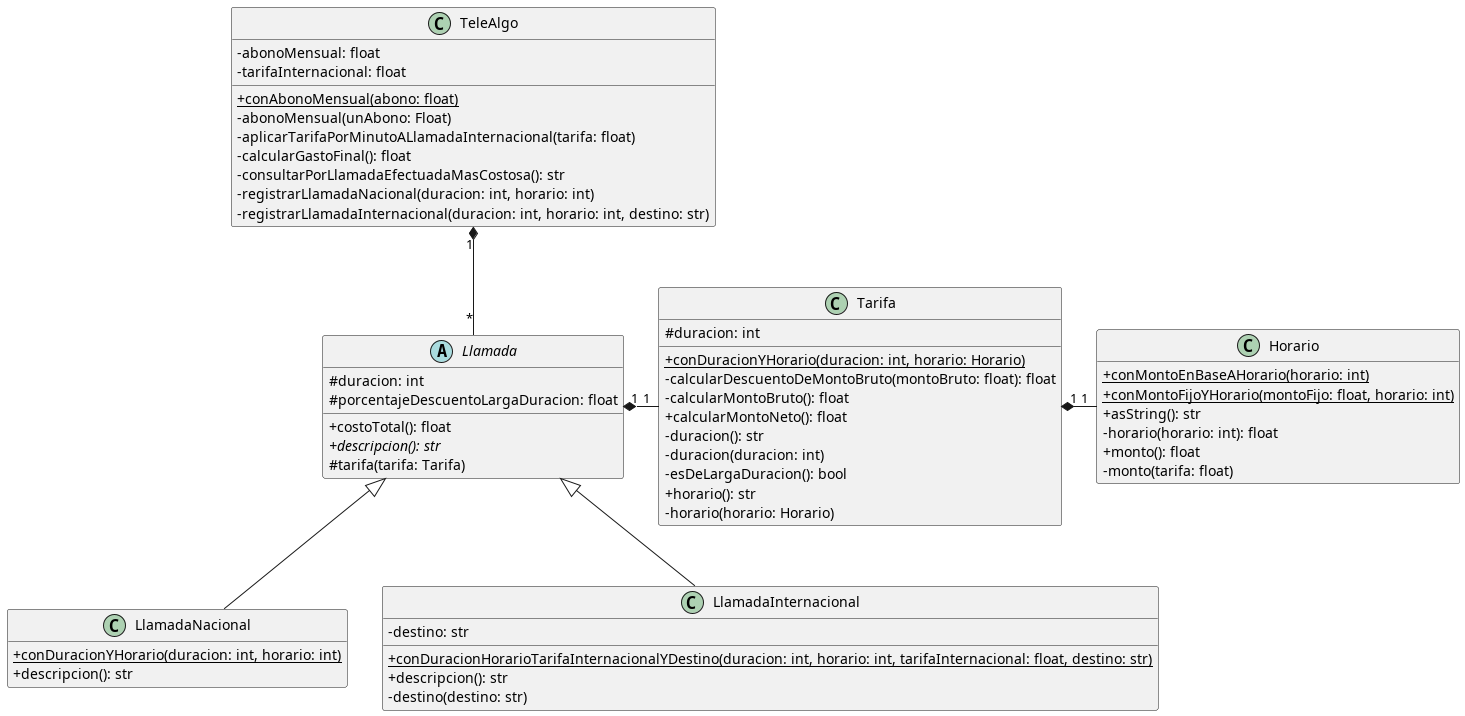
\includegraphics[width=0.85\textwidth]{completo.png}
\caption{\label{fig:class01}Diagrama de clases.}
\end{figure}

\subsection{Diagramas con excepciones}

\begin{figure}[H]
\centering
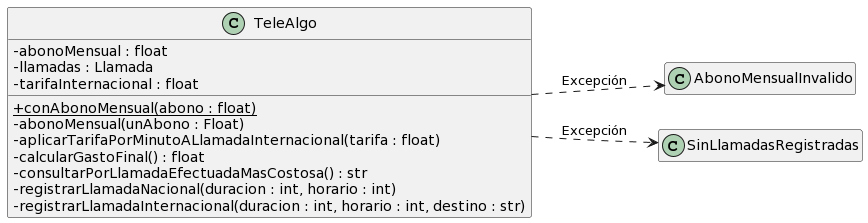
\includegraphics[width=0.8\textwidth]{Excepciones_TeleAlgo.png}
\caption{\label{fig:class02}Excepciones utilizadas por TeleAlgo}
\end{figure}

\begin{figure}[H]
\centering
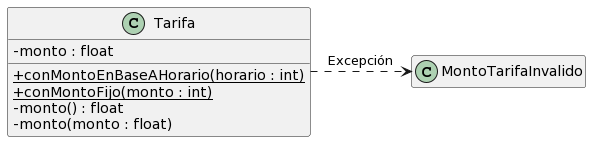
\includegraphics[width=0.8\textwidth]{Excepciones_Tarifa.png}
\caption{\label{fig:class03}Excepciones utilizadas por Tarifa}
\end{figure}

\begin{figure}[H]
\centering
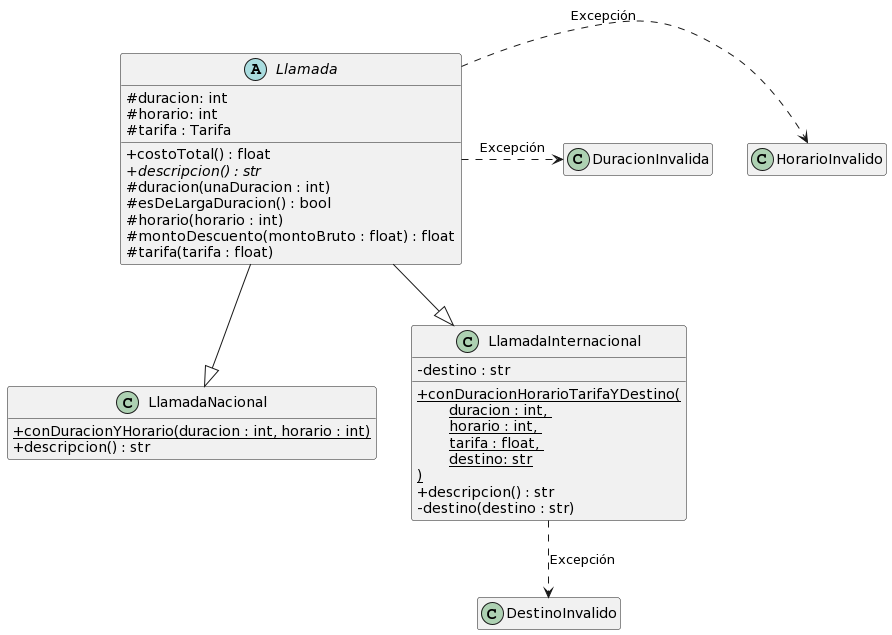
\includegraphics[width=0.8\textwidth]{Excepciones_Llamada.png}
\caption{\label{fig:class04}Excepciones utilizadas por Llamada}
\end{figure}



\section{Excepciones}\label{sec:excepciones}
% Explicación de cada una de las excepciones creadas y con qué fin fueron creadas.

\begin{description}
\item[AbonoMensualInvalido] Se lanza desde la clase \lstinline{TeleAlgo} cuando se intenta crear un teléfono con una cuota de abono mensual con una valor negativo para prevenir que se cree la línea telefónica con este valor incorrecto.
\item[DestinoInválido] Se lanza desde la clase \lstinline{LlamadaInternacional} cuando se intenta crear una llamada internacional con un destino sin nombre. Esto puede suceder porque al setter de este atributo se le puede enviar una string vacía, pero esto no indicaría ningun destino concreto para la llamada internacional. 
\item[DuracionInvalida] Se lanza desde la clase \lstinline{Llamada}, directamente desde el setter del atributo \lstinline{duracion} para prevenir que se creen llamadas con duración negativa.
\item[MontoTarifaInvalido] Se lanza desde la clase \lstinline{Tarifa} cuando se intenta crear una tarifa con monto negativo. El caso en el que la tarifa podría ser igual a cero es que las llamadas sean gratuitas.
\item[SinLlamadasRegistradas] Se lanza desde la clase \lstinline{TeleAlgo} cuando se intenta encontrar la llamada mas costosa en una colección de llamadas que está vacía, en dicho caso no tiene sentido encontrar la llamada más costosa porque ni siquiera existe.
\end{description}



\section{Diagramas de secuencia}\label{sec:diagramasdesecuencia}
% Mostrar las secuencias interesantes que hayan implementado. Pueden agregar texto para explicar si algo no queda claro.

\begin{verbatim}
| rango |
rango := (2 to: 20) asOrderedCollection.
Transcript show: rango ; cr.
rango copy do: [ :unNumero | unNumero isPrime ifFalse: [ rango remove: unNumero ] ].
Transcript show: rango.
\end{verbatim}

\begin{figure}[H]
\centering
\includegraphics[width=\textwidth]{diagrama_secuencia02.png}
\caption{\label{fig:seq02}Nam a nulla non mauris ullamcorper.}
\end{figure}

\end{document}
